\documentclass{article}

% to give various notational syntax
\usepackage{amsmath,amsthm,amssymb, mathtools, enumerate, physics}

% for including images
\usepackage{graphicx}
\graphicspath{ {../../Images/} }
% Resize figures that are too wide for the page.
\makeatletter
\def\ScaleIfNeeded{%
  \ifdim\Gin@nat@width>\linewidth
    \linewidth
  \else
    \Gin@nat@width
  \fi
}
\makeatother
\let\oldincludegraphics\includegraphics
\renewcommand\includegraphics[2][]{%
  \oldincludegraphics[width=\ScaleIfNeeded]{#2}
}
%
%% for bibliography and citation
%\usepackage[square,compress]{natbib}
%\setcitestyle{super,comma}
%\bibliographystyle{unsrtnat}
%
%% for executing and including python code
%\usepackage{pythontex}
%
%% for defining lovely colors
%\usepackage{xcolor}
%\definecolor{light-gray}{gray}{0.95}
%
%% for syntax highlighting of non-python languages
%\usepackage{minted}
%\usemintedstyle[cpp]{manni}
%\newcommand{\cpp}[1]{\mintinline{cpp}{#1}}

% for linking sections of the document and table of contents
\usepackage{hyperref}
\hypersetup{
    colorlinks=true, %set true if you want colored links
    linktoc=all,     %set to all if you want both sections and subsections linked
    linkcolor=blue,  %choose some color if you want links to stand out
}


\newcommand{\nn}{\newline\newline}
\newcommand{\n}{\newline}
\newcommand{\bq}{\begin{equation}}
\newcommand{\eq}{\end{equation}}
\newcommand{\ba}{\begin{align}}
\newcommand{\ea}{\end{align}}
\newcommand{\bi}{\begin{itemize}}
\newcommand{\ei}{\end{itemize}}
\newcommand{\ct}[1]{\citep{#1}}

\newcommand*{\Perm}[2]{{}^{#1}\!P_{#2}}
\newcommand*{\Comb}[2]{{}^{#1}C_{#2}}




\begin{document}

\title{Random Variables and Law of Large Numbers}
\date{}
\maketitle

\textbf{Question:} What is a random variable or vector? Define the two main distributions of interest over the elements of a random \textit{vector}.\n

\textbf{Problem:} We toss a coin 3 times, and define X = number of heads on first toss (0 or 1) and Y = total number of heads in all 3 tosses. What is the marginal distribution of Y? What is the conditional distribution of Y given that X = 0? It is helpful to draw a table.\n

\textbf{Question:} How do you find PDFs of RVs that are functions of other RVs whose PDFs are already known?\n

\textbf{Problem:} Find the probability density of the RV $Y$ given that you know that $Y=X^2$ and $X\sim U(-1,1)$.\n

\textbf{Question:} What are the Expectation (mean) and Variance of a random variable? What is the expectation of a \emph{function} of a random variable? What is the Covariance of two RVs?\n

\textbf{Question:} What is the \emph{Correlation} between two random variables, and how is its value affected by the nature of the joint distribution.\n

\textbf{Problem:} Derive the properties of the sample mean RV for an $n$-sized sample.\n

\textbf{Problem:} Define $Y = g(U) =U^2$ where $U \sim U(0,1)$ . Find $E(Y)$ directly from the definition, and then using the shortcut for mean of a function of an RV.\n

\textbf{Problem:} Find the expecation and variance of a binomially distributed RV using an indicator variable approach.\n

\textbf{Question:} Define conditional expectation. Derive the Law of Total Expectation.\n

\textbf{Problem:} In a game show a person is brought into a room with 3 unmarked doors. Door1 leads to safety in 3 minutes, Door2 circles back into the room in 5 minutes, and Door3 circles back into the room in 7 minutes. Each time the person arrives in the room he is disoriented before choosing a door. What is the expected time it takes him to reach safety?\n

\noindent
\textbf{Problem:} Find the mean of the geometric distribution.\n

\noindent
\textbf{Question:} What is the Law of Large Numbers? Prove Markov's Inequality.\n


\vspace{.3 in}

\tableofcontents

\section{Random Vectors and Joint Distributions}
\textbf{A random variable (RV) is a function defined on a samples space}. It is intuitively described as a numerical feature or description of a random outcome. Consider the sample space of outcomes where a trial consists of tossing a coin three times. There are 8 outcomes in this sample space, and an RV might be defined as the number of heads in an outcome. 
\nn
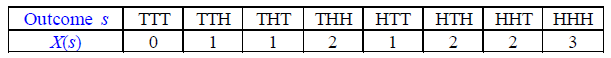
\includegraphics{rv}
\nn

The distribution of an RV stems from the underlying distribution of the outcomes. An RV is called discrete if it can take on only finitely many or countably infinitely many values, otherwise it is continuous. The distribution of a discrete RV is given by a list of the possible values of the random variable together with the probabilities that the RV takes on those values - this is a \textbf{probability mass function}.
\nn

A \textbf{random vector} is a vector of random variables (that may or may not be dependent), and the probability distribution of a random vector is a \textbf{joint distribution}. 
\begin{equation}
f_{X_1,...X_n}(x_1,...x_n) = P\{(X_1,...X_n)=(x_1,...x_n)\}
\end{equation}
The \textbf{marginal distribution} $f_{X_1}(x_1)$ of one of the random variables in the vector gives the probability of that value of the random variable occuring, without reference to the values of the other variables. If you are looking at the joint distribution you should picture transferring the probability mass at every point of the joint distribution onto the corresponding values along the $X_1$ dimension (so transfer it along a line orthogonal to the $X_1$ dimension). 
\nn

The \textbf{conditional distribution} of $X_1$ gives the probability to measure different values of $X_1$ given that another variable (or variables) of the random vector took on certain values. This distribution can be pictured as taking a slice of the joint distribution along the direction in which the conditional values occur. For example, in a two-dimensional joint distribution the conditional distribution $f_{X_1|X_2}(x_1|x_2)$ would be proportional to the slice of the joint density along the line $X_2 = x_2$. 
\nn

In terms of actually computing these two distributions in the two-dimensional (discrete) case:
\begin{align}
f_X(x) = \sum_y f_{X,Y}(x,y)\\
f_{X|Y}(x|y) =  \frac{f_{X,Y}(x,y)}{f_Y(y)}
\end{align}



\subsection{Problem: Coin Toss Joint Distribution}
The marginal distribution for Y on the outcome set $\{0, 1, 2, 3\}$ is $\{\frac{1}{8}, \frac{3}{8},\frac{3}{8},\frac{1}{8}\}$. The conditional distribution for Y given X = 0 over the same outcome set is $\{\frac{1}{4}, \frac{1}{2},\frac{1}{4},0\}$. Notice how the probability mass has shifted to the lower values of Y.


\section{Transformations of RVs and Associated Probability Densities}
We often want to know the pdf for an RV which is a function of another RV whose pdf is already know. There are two ways to get at this - through the relationship of the PDFs or through the relationship of the CDFs. We first describe the former.
\n

Consider two random variables $X$ and $Y$ that satisfy the relationship $Y=g(X)$ - this expression is a mapping between their two spaces. The first step in determining the pdf of one RV from that of another, is to carefully consider this mapping and whether it is one-to-one. For example,for $Y=X^2$ the value $Y=1$ actually maps back to two points in $X$-space: +1 and -1. So here a single neighborhood around $Y=1$ with a certain probability weight, actually corresponds to two neighborhoods in $X$-space, around +1 and around -1, whose probability weights will add up to the weight of the $Y$-neighborhood:
\begin{align*}
 P\bigg(\textrm{$Y$ within some neighborhood about 1}\bigg) =\\
 P\bigg(\substack{\text{$X$ within corresponding    }\\\text{neighborhood about +1    }}\text{OR }\substack{\text{ $X$ within corresponding}\\\text{neighborhood about -1}}\bigg) =\\
  P\bigg(\substack{\text{$X$ within corresponding}\\\text{neighborhood about +1}}\bigg) + P\bigg(\substack{\text{ $X$ within corresponding}\\\text{neighborhood about -1}}\bigg).
 \end{align*}
Let's first walk through the idea of extracting the pdf assuming the mapping is 1:1 and then return to this more complicated example. Consider the following general case where we are given $Y=g(X)$ and we know the pdf $f_X(X=x)$. The pdf of a continuous variable $Y$ is defined as the function $f_Y$ that achieves:

\begin{align*}
P\bigg(\textrm{$Y$ within some $\Delta Y$ of $y_0$}\bigg) \approx f_Y(y_0)\Delta Y,
\end{align*}
as we shrink $\Delta Y$. Since there is a mapping between our two RVs we know that this neighborhood within $\Delta Y$ of $Y=y_0$ is associated with a corresponding neighborhood in $X$-space centered around $X=g^{-1}(y_0)=x_0$ which receives the same probability weight:
\begin{align*}
P\bigg(\textrm{$Y$ within some $\Delta Y$ of $y_0$}\bigg) = P\bigg(\textrm{$X$ within some $\Delta X(\Delta Y)$ of $g^{-1}(y_0)$}\bigg).
\end{align*}
Here the size of the $\Delta$ in $X$-space is a function of the sizeof $\Delta$ in $Y$-space. As we shrink the $Y$-neighborhood closer about $y_0$ the relationship approaches
\begin{align*}
f_Y(y_0)=f_X(x_0)\frac{dX}{dY}\bigg|_{y_0} = f_X(x_0)\frac{1}{\frac{dY}{dX}\bigg|_{X=x_0}} = f_X(x_0)\frac{1}{g'(x_0)},
\end{align*}
where again we remember that $x_0 = g^{-1}(y_0)$. Since we are interested in the probability associated with \textit{areas} of neighborhoods what we really care about is the magnitude of the ratio between the area in $X$ space and the area in $Y$ space, and since we want to keep probabilities positive the true expression to use is
\begin{equation}
f_Y(y_o) = f_X(x_0)\frac{1}{|g'(x_0)|}
\end{equation}
This can be thought of as follows: the probability weight at $Y=y$ is large if the weight at the corresponding point $x=g^{-1}(y)$ is large, but also if the mapping in the region of $y$ tends to stretch $Y$-space over larger areas of $X$-space so as to capture more weight i.e. $|\frac{\Delta Y}{\Delta X}|\big(=|g'(X)|\big) \leq 1$.
\n

This method of working with pdfs generalizes nicely to transformations involving more than one RV. Consider RVs $U$ and $V$ which map to RVs $X(U,V)$ and $Y(U,V)$. Refer to the image below: if we imagining forming a neighborhood in $U,V$ space about the point $(u,v)$ it will cover an area $R=(du)(dv)$ and will map to some corresponding region in $X,Y$ space about the point $(x(u,v),y(u,v))$ and covering area S. The relationship between R and S is illustrated by the parallelogram in the figure. The parallelogram cirsumscribes all the $(x,y)$ points that are mapped by allowing $U$ and $V$ to vary independently over the entire neighborhood R. The area of the parallelogram is given by the magnitude of the cross product of the two vectors forming the two sides of the acute angle. This in turn can be written as the product of the determinant of a matrix (which is given the special name of Jacobian) with the area $dudv$.

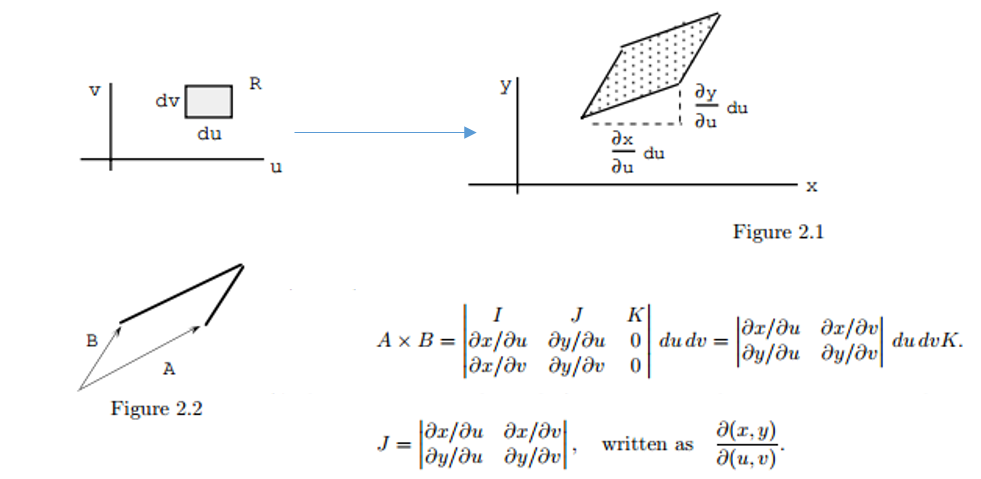
\includegraphics{jacobian.png}

So we have $S = |\vec{A}\times\vec{B}| = |\frac{\delta(x,y)}{\delta(u,v)}|dudv$, and in analogy with the one-dimensional case before, we then have the balance of the probability weightings between the two neighborhoods: 
\begin{align*}
f_{XY}(x(u,v),y(u,v))|J|dudv = f_{UV}(u,v)dudv \\
\implies f_{UV}(u,v) = \frac{f_{XY}(x(u,v),y(u,v))}{|\frac{\delta(u,v)}{\delta(x,y)}|}.
\end{align*}
In the last step we have used a convenient property Jacobians. Refer to the excellent notes at \url{http://www.math.uiuc.edu/~r-ash/Stat/StatLec1-5.pdf} for more information. 
\n
 
The other common method is to first find the CDF of the second RV using the inverted mapping, and then to differentiate the CDF.  For example, in the laser pole problem where $X=tan(A)$ we know from picturing the tangent function that as $A$ decreases from 90 to -90 degrees, it gets mapped one-to-one to a value of X in a monotonically decreasing fashion. So we know that if $X$ is greater than some value $x$, it guarantees that $A \geq tan^{-1}(x)$. In terms of the CDFs, $F$, we then say:
\begin{equation}
F(x) = P(X \leq x) = P(tan(A) \leq x) = P(A \leq tan^{-1}(x)).
\end{equation}
The final quantity we can calculate since we know the density and thus the CDF of $A$. We would then differentiate $F(x)$ to obtain the densty $f(x)$. The actul result for this case is given the laser pole problem. 
\n


\subsection{Problem: PDFs of $Y=X^2$ Knowing $X$-distribution.}
Refer to the notecard on RVs for a general discussion of getting the pdf for an RV which is a function of another RV whose pdf you already know. For the case $Y=X^2$ we can say:
\begin{align*}
F(y) = P(Y \leq y) = P(X^2 \leq y) = P(|X| \leq \sqrt y) \\
= P( -\sqrt y \leq X \leq \sqrt y)=2\sqrt{y}  \frac{1}{2},
\end{align*}
Where we have used our knowledge of the uniform density (which is symmetric) to actually evaluate the probability of this interval. In general you would use the analytical form of the CDF for $X$ which you can obtain from the known pdf. Now we have the CDF of $Y$ and can differentiate to obtain the desired pdf,
\begin{equation}
f(y) = F'(y) = \frac{d}{dy}\sqrt{y}=\frac{1}{2}y^{1/3}.
\end{equation}



\section{Expectation and Variance of RVs}
Let X be a discrete random variable taking values $x_i$ with probabilites $p_i$, then the \textbf{expectation} or \textbf{mean} of this random variable is 
\begin{align}
\mathrm{E} [X]=\sum _{\text{all SS}}x_{i}\,p_{i} \\
\text{( }\mathrm{E} [X]=\int _{-\infty }^{\infty }xf(x)\,\mathrm {d} x \text{ for continuous RV).}
\end{align}
Expectations obey linearity, and have a nice product rule for independent RVs:
\begin{align}
\mathrm {E}[X+Y] = \mathrm{E}[X] + \mathrm{E}[Y]\\
\text{X, Y independent }\implies \mathrm {E}[XY] = \mathrm{E}[X]\mathrm{E}[Y].
\end{align}
The \textbf{mean of a function of an RV} (which is itself a random variable) can be calculated in shortcut fashion rather than from the definition. If $X$ is an RV with pmf $f(x)$, then $\mathrm {E} [g(X)]=\int _{-\infty }^{\infty }g(x)f(x)\,\mathrm {d} x.$
\nn


The \textbf{Variance} gives an idea of how much the RV is spread away from it's mean, $\mu$. Useful properties include:
\begin{align}
\mathrm{Var}(X) \equiv E[(X-\mu)^2] = E[X^2]-(E[X])^2\\
\mathrm{Var}(cX) = c^2\mathrm{Var}(X)\\
\mathrm{Var}(c+X) = \mathrm{Var}(X) \text{  (since the distribution is just shifted)}\\
\mathrm{Var}(X +Y) = \mathrm{Var}(X) + \mathrm{Var}(Y) + 2 \mathrm{Cov}(X,Y)\\
\text{X, Y independent }\implies \mathrm{Var}(X +Y) = \mathrm{Var}(X) + \mathrm{Var}(Y)
\end{align}
An analogue of the last property is that if two vectors are orthogonal then the squared length of the sum is the sum of the squares - and the variance is a squared euclidean distance or length. 
\nn

If the \textbf{Covariance} of $X$ and $Y$ is zero, then they are said to be \textbf{uncorrelated} but note that it does not imply independence. The intuition for covariance is that it will be large if the distributions behave similarly once they have both been shifed so their means are at 0.
\begin{equation}
\mathrm{Cov}(X,Y) \equiv \mathrm{E}[(X-\mu_x)(Y-\mu_y)]
\end{equation}
\nn

\subsection{Correlation}
First lets consider a constraint that exists on any two variables $W$and $Z$, namely that the expectation value for the product random variable, $E[WZ] = \int{wzf(w,z)dwdz}$, is a generalized dot product and satisfies a triangle inequality: 
\begin{align*}
E[WZ] \leq \sqrt{E[W^2]E[Z^2]} \\
\implies \mathrm{Cov}(W,Z) = E[(W-\mu_W)(Z-\mu_Z])] \leq \sqrt{E[(W-\mu_W)^2]E[(Z-\mu_Z)^2]}\\
\implies \frac{\mathrm{Cov}(W, Z)}{\sqrt{\mathrm{Var}(W)\mathrm{Var}(Z)}} \leq 1
\end{align*}

This last quantity is called the \textbf{Correlation }, $\rho$, and it is a measure of the strength of a linear relationship between two variables. Correlation approaches 1 the more a random sample from the joint distribution $(W, Z)$ tends to return a pair with $W$ positioned similarly relative to $\mu_W$ as $Z$ is relative to $\mu_Z$. Obviously as $W$ and $Z$ approach independence this tendency will go to zero. Sample correlation is just calculating an estimate of this quantity using the naive sample variance and sample covariance estimators. The correlation actually appears in the analytical form of the least-squares regression line for a first order linear model (discussed in the estimation review card).

\subsection{Problem: Mean \& Var of Sample Mean}
If you draw a set of values $\{X_1, X_2,... X_n\}$  from an underlying disribution with mean $\mu$ and standard deviation $\sigma^2$ such that each value is independently drawn, you have a \textbf{random sample} and the average of the values in the sample, $\bar{X}$, is called the \textbf{sample mean}. An $n$-sized sample is a random vector with a certain joint distribution, and the sample mean is a RV over this distribution. We can make certain statements about this RV:
\begin{align}
\bar{X} \equiv \frac{1}{n}\sum_{i=1}^n X_i\\
\mathrm{E}[\bar{X}] = \mu\\
\mathrm{Var}(\bar{X}) = \frac{\sigma^2}{n}
\end{align}
This means that if you draw a large sample (large $n$) then you can be more certain that the average value you calculate from that sample is close to the mean of the generating distribution $\mu$. This is the idea of the LLN discussed below.



\subsection{Problem: Mean of Functions of RVs}
To use the definition of expectation we need the density of Y. 
\begin{align}
F_Y(y) = P\{U^2 \leq y\} = P\{U \leq y^{1/2}\} = y^{1/2}\\
f_Y(y) = \frac{d}{dy}F_Y(y) = \frac{1}{2}y^{-1/2}\\
\mathrm {E} [Y]=\int y f(y)\,\mathrm {d} y = \int _{0}^{1}\frac{1}{2}y^{1/2}dy = \frac{1}{3}
\end{align}
On the other hand, the RV of interest is a function of another RV which we already know the density of, so we can just say:
\begin{equation}
\mathrm {E} [g(U)]=\int g(u)f(u)\,\mathrm {d} u = \int _{0}^{1}u^2du = \frac{1}{3}
\end{equation}



\subsection{Problem: Mean \& Var of Binomial Distribution and Indicators!}
An \textbf{Indicator} RV is a binary RV which signals the occurence of an event, A, by mapping $I(A) = 1$ if $A$ occurs, and 0 otherwise. Recasting problems in terms of indicator variables can simplify things. 
\nn

A brute force approach to finding $\mathrm{E}[K\sim B(n,p)]$ would involve doing the sum: $E[K] = \sum_{k=1}^{n}{n\choose k}  p^k(1-p)^{n-k}.$ But we can instead think of our binomially distributed RV as a sum of indicator RVs: $K = I_1 + I_2... I_n$ and apply the linearity of expecation. 
\begin{equation}
E[K] = \sum_{i=1}^{n}E[I_i] = n[1(p)+0(1-p)] = np,
\end{equation}
since all the trials of a binomial RV are identical and independent. The decomposition of $K$ into a sum of indicators also helps with the variance - since the $I_i$'s are independent the Variance of their sum obeys linearity:
\begin{equation}
\mathrm{Var}(K) = \sum_i \mathrm{Var}I_i = n[(1-p)^2(p)+(0-p)^2(1-p)] = np(1-p)
\end{equation}



\section{Conditional Expectation}
A conditional expectation on $Y$ given an event $A$ gives a mean or expected value of $Y$ assuming we are drawing from a particular region of the joint distribution (the region of event $A$). It is defined as
\begin{equation}
\mathrm{E}[Y | A] = \sum_y y\mathrm{P}(Y=y | A).
\end{equation}
The probabilities in the sum are given by the conditional distribution for $Y$. Similarly to normal expectation, a conditional expectation of a function of a RV can be calculated by a shortcut method
\begin{equation}
\mathrm{E}[g(Y) | X=x] = \sum_y g(y)\mathrm{P}(Y=y | X=x)
\end{equation}
The law of total probability along with the definition of a conditional expectation can be used to generate the \textbf{Law of Total Expectation} which partitions the sample space and first calculates an expectation in each partition before then taking a weighted average of the partition expectations.
\begin{equation}
\mathrm{E}[Y] = \sum_xP(X=x)\mathrm{E}[Y | X=x]
\end{equation}



\subsection{Problem: Gameshow Maze (condition on initial state)}
The RV $T$ is the total time to get to safety and it is defined over a sample space that consists of all the possible sequences of choices. Using the brute force definition we would need the probabilities of all these sequences and their $T$-value. Instead we will use a \textbf{generally useful trick which is to partition by (AKA \textit{condition on}) the initial state}. Call the initial door choice the RV $R$, parititioning by this RV and using the Law of Total Expectation we can say
\begin{equation}
\mathrm{E}[T] = \sum_r=1^3 P(R=r)\mathrm{E}[T | R=r] = (\frac{1}{3})(3) + (\frac{1}{3})\mathrm{E}[T | R=2] + (\frac{1}{3})\mathrm{E}[T | R=3]
\end{equation}
Now picture all the sequences that fall in the $R=2$ partition - the contestant has chosen Door2 and spent 5 minutes to get back to the room. But now that he is in the room he's in exactly the same position he was in initially - no information and standing in the room. So logically the sample space that is the remaining sequence of his choices should look identical to the full sample space and thus should have the same expectation of $T$. So by symmetry we believe that $\mathrm{E}[T | R=2] = 5 + \mathrm{E}[T]$. Applying this logic to the Door3 partition as well, we have
\begin{equation}
\mathrm{E}[T] = = (\frac{1}{3})(3) + (\frac{1}{3})(5+\mathrm{E}[T]) + (\frac{1}{3})(7+\mathrm{E}[T] \implies \mathrm{E}[T] = 15
\end{equation}



\subsection{Problem: Mean of Geometric Distribution}
Given $T\sim Geom(p)$ we can think of $T$ as a sum of indicator variables: $T = \sum_{i=1}^k I_i$, where all $I_i=0$ except the last one. The sample space is all the possible sequences of 0's truncated with a single 1. We can again use the trick of conditioning on the value of the first indicator variable $I_1$, and then noting that if the first indicator is 0, the expectation for the remainder of the sequence be identical to the expectation of the full sequence. 
\begin{equation}
\mathrm{E}[T] = (p)\mathrm{E}[T | I_1=1] + (1-p)\mathrm{E}[T | I_1=0] = (p)(1)+(1-p)\mathrm{E}[T] \implies \mathrm{E}[T] = 1/p
\end{equation}




\section{LLN and Markov's Inequality}
The \textbf{Law of Large Numbers} says that as you increase your samples size of an RV it becomes more and more likely that the sample mean will be close to the mean of the RV's distribution.

\theoremstyle{plain}
\newtheorem*{lln}{LLN}
\begin{lln}
Let $X_1, X_2,...$ be iid with mean $\mu$ and variance $\sigma^2$ and define $\bar{X}_n = \frac{1}{n}\sum_{i=1}^nX_i$. Then ${\overline {X}}_{n}\ {\xrightarrow {P}}\ \mu  {\textrm {  when}}\ n\to \infty$. 
\end{lln}
Here the P means converges in probability, which means that the probability of an unusual outcome becomes smaller and smaller as the sequence progresses.
\n

The proof of the LLN can be done using the \textbf{Markov Inequality} which gives a bound on the probabiliy that a non-negative RV exceeds a chosen value $a$. 
\newtheorem*{markov}{Markov Inequality}
\begin{markov}
If $X$ is any nonnegative integrable random variable and $a > 0$, then $\mathbb{P}(X \geq a) \leq \frac{\mathbb{E}(X)}{a}$.
\end{markov}

Consider transferring all the probability mass above $a$ to exactly on $a$, and all the probability mass below $a$ to the value 0. In this case the expecation would be $\mathrm{E}(X) = 0\mathrm{P}(X<a)+a\mathrm{P}(X\geq a).$ But as soon any probability mass gets shifted rightward this will increase the expectation, so we have a bound for the expectation as $\mathrm{E}(X)\geq \mathrm{P}(X\geq a)$. Here is a tighter proof using a powerful general technique. 
\begin{proof}[Proof of Markov's Inequality]
Consider a sample space $\Omega$ with elements $\omega_i$, and RV $X$ defined on $\Omega$. Define two new RV's: $X/a$ and $\{X\geq a\}$ where the latter takes value 1 when the statement holds and 0 when it doesn't hold. For all $\omega_i$ in $\Omega$ if $a > 0$ we are guaranteed
\begin{align}
\frac{X}{a} \geq \{X\geq a\} \\
\implies \frac{\mathrm{E}[X]}{a} \geq \mathrm{E}[\{X\geq a\}]
\end{align}
The first line is an \textbf{inequality that holds pointwise over the sample space - constructing these is a good general technique}. The second part  follows because expectation is a monotonically increasing function of the sample space. But the expectation of an indicator is the probability of the event so
\begin{equation} 
\frac{\mathrm{E}[X]}{a} \geq \mathrm{P}(X\geq a)
\end{equation}
\end{proof}
 \textbf{Chebyshev's Inequality} is a special case of the Markov inequality applied to the RV of $(X-\mathrm{E}[X])^2$.


\end{document}